\documentclass[12pt]{article}

\usepackage{pablo-devoir}
%\usepackage{pablo-listings}
\usepackage[a5paper,margin=1cm]{geometry}

\pagestyle{empty}

\title{Fonctions Statistiques}
\date{14/01/15}
\classe{2\up{des}14}
\dsnum{DS 4}

\begin{document}
\textbf{\Large Nom : \ldots\ldots\ldots\ldots\ldots\ldots\ldots\ldots\ldots}
\vspace{.5cm}

\maketitle

\begin{exercice}[Fonctions affines --- 4 points]~
  On considère deux fonctions $f:x\mapsto -0,5x+6$, et $g:x\mapsto 2x-4$,
  définies sur l'ensemble des réels $\mathbb{R}$.
  \begin{enumerate}
    \item Donner les variations de $f$ et $g$ sur leur ensemble de définition.
    \item Calculer $f(4)$ et $g(4)$.
    \item Comparer, \emph{sans nouveaux calculs}, $f(10)$ et $g(10)$.
  \end{enumerate}
\end{exercice}

\begin{exercice}[Compétition --- 3 points]
  Voici les scores obtenus dans une compétition de tir à l'arc par
  les 40 joueuses.

  \begin{tabular}{c||c|c|c|c|c|c|c|c|c|c}
    Score
    & 400
    & 410
    & 433
    & 442
    & 453
    & 460
    & 478
    & 483
    & 492
    & 498
    \\
    \hline
    Effectif
    & 2
    & 4
    & 2
    & 8
    & 5
    & 7
    & 5
    & 4
    & 1
    & 2
    \\
    \hline
    &&&&&&&&&&
  \end{tabular}

  \begin{enumerate}
  \item Calculer la médiane et les quartiles de cette série.
  \item L'an passé, la moitié des candidates avait obtenu un score inférieur à
    440. À l'aide de cette seule information, peut-on dire que le niveau des
    joueuses a plutôt augmenté ou plutôt baissé ?
  \end{enumerate}

\end{exercice}

\begin{exercice}[Échantillonnage --- 6 points]~
  \noindent\emph{Les deux questions sont indépendantes.}

  Travaillant dans un laboratoire de contrôle pharmaceutique, vous êtes chargé(e) d'étudier deux traitements $A$ et $B$, censés guérir une certaine maladie. On sait que pour cette maladie, 30\% des malades guérissent spontanément (c'est-à-dire sans médicament) en moins d'une semaine. La question à laquelle vous devez répondre est : Ces médicaments permettent-ils une guérison plus rapide ?

  \begin{enumerate}
    \item Testé auprès de 30 personnes, le traitement $A$ en a guéri 17 en moins d'une semaine. On note $p_A$ la proportion théorique de malades guérissant en moins d'une semaine avec le médicament $A$.
      \begin{enumerate}
        \item Déterminer un intervalle de confiance à 95~\% de $p_A$, donné par la formule $\left[f-\frac{1}{\sqrt{n}};f+\frac{1}{\sqrt{n}}\right]$, où $f$ est la fréquence des guérisons de l'échantillon en moins d'une semaine, et $n$ la taille de l'échantillon.
        \item Pouvez-vous affirmer que ce médicament accélère le temps de guérison ? Justifier.
      \end{enumerate}
    \item Un intervalle de confiance à 95~\% de la proportion $p_B$ de guérisons en moins d'une semaine avec le traitement $B$ est $\left[0,27;0,41\right]$. Pouvez-vous affirmer que ce traitement accélère la guérison ? Justifier.
  \end{enumerate}
\end{exercice}

\begin{exercice}[Résolution graphique d'(in)équations --- 6 points]
  On considère les fonctions $f$ et $g$, définies sur $\left[ -4;6 \right]$ et
  représentées sur le graphique suivant.
  \begin{center}
    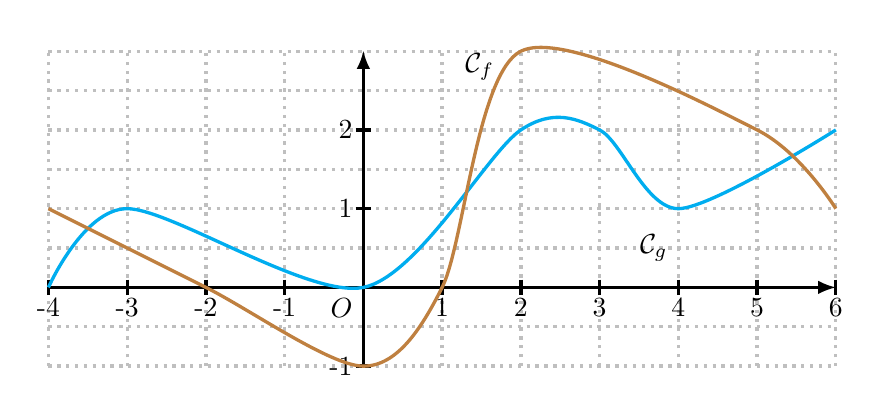
\begin{tikzpicture}[very thick,xscale=1, yscale=1]
      \draw[dotted, lightgray, xstep=1, ystep=.5] (-4, -1) grid (6, 3);
      \draw[-latex] (-4,0) -- (6,0);
      \draw[-latex] (0,-1) -- (0,3);
      \foreach \x in {-4, -3, -2, -1, 1, 2, 3, 4, 5, 6} {
        \draw (\x,0) node[below]{\x};
        \draw (\x,{0.1}) -- (\x,{-0.1});
      }
      \foreach \y in {-1, 1, 2} {
        \draw (0,\y) node[left]{\y};
        \draw (-.1, \y) -- (.1, \y);
      }
      \draw [cyan] plot [smooth, tension=0.5] coordinates {
        (-4,0)
        (-3, 1.0)
        (0, 0)
        (2, 2)
        (3, 2)
        (4, 1)
        (6, 2)
      };
      \draw [brown] plot [smooth, tension=0.5] coordinates {
        (-4,1)
        (-2, 0)
        (0, -1.0)
        (1, 0)
        (2, 3)
        (5, 2)
        (6, 1)
      };
      \draw (0,0) node[below left]{$O$};
      \draw (1.8, 2.8) node[left]{$\mathcal{C}_f$};
      \draw (4.0, 0.5) node[left]{$\mathcal{C}_g$};
    \end{tikzpicture}
  \end{center}
  \emph{Répondre aux questions par lecture graphique.}
  \begin{enumerate}
    \item Déterminer les solutions de $f(x)<0$
    \item Déterminer les solutions de $f(x)\geq g(x)$.
    \item Tracer la courbe d'une fonction $h$ telle que les solutions de $h(x)>f(x)$ soient $\left[ -4;1 \right[ \cup \left] 4;5 \right[$.
      \item Pourquoi n'existe-t-il pas de fonction $p$ telle $p(x) \geq g(x)$, et $p(x)\leq0$ sur $\left[ 2;4 \right]$ ?
  \end{enumerate}

\end{exercice}

\begin{exercice}[Moyenne --- 1 points]
Un élève a une moyenne de 9 à trois devoirs. Quelle note minimale devra-t-il avoir au prochain devoir pour que sa moyenne soit au moins égale à 10 ?
\end{exercice}

\end{document}
